\documentclass[a4paper]{scrartcl}
\usepackage[utf8]{inputenc}
\usepackage[english]{babel}
\usepackage{graphicx}
\usepackage{lastpage}
\usepackage{pgf}
\usepackage{wrapfig}
\usepackage{fancyvrb}
\usepackage{fancyhdr}
\pagestyle{fancy}

\usepackage[backend=bibtex, citestyle=numeric-comp, bibstyle=ieee]{biblatex}
\addbibresource{ref.bib} % The file containing our references, in BibTeX format
\usepackage{hyperref}
\usepackage{listings}
\usepackage{subcaption}

% Create header and footer
\headheight 27pt
\pagestyle{fancyplain}
\lhead{\footnotesize{Internet Applications, ID1354}}
\chead{\footnotesize{Tasty Recipes with HTML and CSS}}
\rhead{}
\lfoot{}
\cfoot{\thepage\ (\pageref{LastPage})}
\rfoot{}

% Create title page
\title{Tasty Recipes with HTML and CSS}
\subtitle{Internet Applications, ID1354}
\author{Julius Recep Colliander Celik - jcelik@kth.se}
\date{\today}

\begin{document}

\maketitle

%\section*{Tips for Report Writing}
%\textbf{REMOVE THIS SECTION BEFORE SUBMITTING THE REPORT.}\\
%
%\noindent \textit{The target audience has exactly the same skills as the author, except they do not know anything at all about the specific program described in the report.} \\
%
%Consider the following:
%
%\begin{itemize}
%  \item \textbf{The report must be \textit{centered around the requirements}. Which are they (Introduction), how did you work to meet them (Method), what is the solution that meets them (Result), and how can you be sure they are met (Discussion). This is the IMRaD method.}
%
%  \item \textbf{The report must show that you have done the work yourself and that you have understood what you have done. Both of these goals are met by carefully explaining the source code.}
%
%  \item Is spelling and grammar correct? Is spoken language avoided?
%
%  \item Does the report have a good structure with sections, subsections and paragraphs?
%
%  \item Is the solution clearly explained? Will the reader understand the program? What would you yourself want to know if you read about the program, is that included in the report?
%
%  \item Is the solution analyzed and evaluated? Are important properties of the program explained? Should there have been more extensive evaluation?
%
%  \item Is the text clarified with images and/or other figures, and with links to the code in your Git repository? Remember that all figures (images, tables, graphs, code listings, etc) shall be numbered and have a short explaining text.
%\end{itemize}

\section{Introduction}

A web site for sharing tasty recipes was created. The goal was to create a web site using only HTML and CSS, following halve of the heuristics of user design, as well as considering accessibility, and preferably being responsive by adapting the web site to different screen sizes. To ensure consistency a CSS reset style sheet had to be used, and to ensure good code quality all files created had to be pass the W3C validations.

The web site created contained of four pages. One home page, two recipe pages, and one calendar page. Every page had to be accessible from any other page, which is why a navigation menu was recommended. To view the website it is publicly available on the link \href{https://github.com/juliuscc/kth-id1354/tree/master/homework-1}{https://github.com/juliuscc/kth-id1354/tree/master/homework-1}. The website is also deployed on the url \href{https://receps-recept.com}{receps-recept.com}, which is a pun based on the similarity between my middle name (Recep) and the Swedish word for recipe (recept).

\section{Literature Study}

The web page w3schools is a web page with extensive information about HTML, CSS and many other web technologies. The web page w3schools was used for basic CSS reference \cite{RefsnesData}. For reference of CSS Flexbox and CSS Grid the complete guides from CSS-Tricks was used \cite{Coyier,Coyiera}. 

For design inspiration, the calendar is visually based on another calendar. A calendar created using the framework Semantic UI was openly shared and was the basis for creating the calendar on the Tasty Recipes web site \cite{Nijin39} . As I have been mostly fluent in HTML and CSS, for the past 4 years prior to this assignment, no other resources were necessary.

\section{Method}
This chapter is divided into two parts. The first part (Chapter \ref{method:development}) explains the tools used and the development environment. It also describes how the web site was publicly published. The second part (Chapter \ref{method:evaluation}) explains how the web page was evaluated. The web site was mostly manually evaluated, however browser compatibility and code validity is discussed in this chapter.

\subsection{Development environment}
\label{method:development}

The text editor used was Visual Studio Code. This decision was based on personal preference, as well as it being the most popular development environment \cite{Stackoverflow}. I considered using SASS with an SCSS syntax, or PostCSS as it helps with structuring projects. After consideration I choose to use only pure HTML and CSS as the project is very small and simple. To keep a good structure on my CSS I used the Block Element Modifier (BEM) methodology. It is a very simple naming methodology that results in very elegant code \cite{Starkov}.

Of course I used a CSS reset style sheet. I used Normalize.css as I have used it before successfully. It is very lightweight and primarily aims at fixing browser bugs and inconsistent behavior, while preserving useful browser defaults. It is used by ``[...] Twitter, TweetDeck, GitHub, Soundcloud, Guardian, Medium, GOV.UK, Bootstrap, HTML5 Boilerplate, and many others'' \cite{Gallagher}.

To deploy the web site I use GitHub Pages, and use CloudFlare for CDN cache and redirection so that the url \texttt{https://receps-recept.com} results in the web site hosted on GitHub Pages being received. For automatic continuous deployment I use Travis CI. For local development I used Browsersync to refresh my browser every time a file was changed. It enabled me to have the web site next to my code and not have to manually refresh the web page every time I made a change in the code.

\subsection{Evaluation}
\label{method:evaluation}

To evaluate  the validity of my code I used the W3C Markup Validation Service. I tested my web site on the following browsers:
\begin{itemize}
	\item Google Chrome - Mac OS X
	\item Firefox - Mac OS X
	\item Safari - Mac OS X
	\item Google Chrome - iOS 12
	\item Opera Mini - iOS 12
	\item Safari - iOS 12
\end{itemize}

This was to ensure that the web site performed consistently over multiple browsers. On the computer I tested both normal view and mobile view in Firefox. The most interesting browser on the list is Opera Mini that is a browser that lacks a large amount of modern features, and purposely ignores certain web features to save battery, internet bandwidth and perform better. It is not always required for the web site to look exactly the same on Opera Mini as it would be limiting for other users, however it is important that the website still is usable on Opera Mini. Internet Explorer and Internet Edge could not be tested as no compatible device was available. However Internet Edge is a browser that often have the latest features, despite Microsoft's history with Internet Explorer being a worse browser than the competitors.

\section{Result (and html head)}

My git repository is found in the following link: \newline\href{https://github.com/juliuscc/kth-id1354/tree/master/homework-1}{https://github.com/juliuscc/kth-id1354/tree/master/homework-1}. The project uses the following file structure:

\begin{verbatim}
|---- icons
|   |---- bars-solid.svg
|   +---- times-solid.svg
|---- images
|   |---- blur-close-up-dairy-product-407041.jpg
|   |---- board-bunch-cooking-349609.jpg
|   +---- emiliano-vittoriosi-703094-unsplash.jpg
|---- calendar.html
|---- index.html
|---- meatballs.html
|---- normalize.css
|---- pancakes.html
+---- style.css
\end{verbatim}

\noindent
It contains four HTML-files which each correspond a page, two CSS style sheets where one is a CSS reset and the other is the web pages style, as well as icons and images.

\subsection{W3C validation and CSS Reset Style Sheet}
The HTML pages and the style sheet were all submitted to the W3C Markup Validation Service. All the four HTML-files and the CSS style sheet showed no errors or warnings. A CSS reset style sheet was used. Normalize.js was the reset style sheet used. It was added in the head before any other style sheets. All pages looked the same on all tested browsers.

\subsection{CSS}
The CSS is written with BEM methodology to make it easier to work with. Here is the link to the file: \href{https://github.com/juliuscc/kth-id1354/blob/master/homework-1/style.css}{https://github.com/juliuscc/kth-id1354/blob/master/homework-1/style.css}. For horizontal alignment i use mostly percentages to ensure that the web site always looks nice. I also use media queries to change the style based on screen size.

Notice row \href{https://github.com/juliuscc/kth-id1354/blob/090d3fcab0dbe83d8e9b82e8ad858ea1843d1ffe/homework-1/style.css#L204}{204} of the file where I use a media query. The media query decides that if the screen width is smaller than 800px the margins get smaller and the two-column grid becomes a one-column grid. This was done with CSS Grid.

On row \href{https://github.com/juliuscc/kth-id1354/blob/090d3fcab0dbe83d8e9b82e8ad858ea1843d1ffe/homework-1/style.css#L225}{225} i specify a transition that is relevant for when a user hovers over a recipe-card. When a user hovers over a recipe-card the block that starts on row \href{https://github.com/juliuscc/kth-id1354/blob/090d3fcab0dbe83d8e9b82e8ad858ea1843d1ffe/homework-1/style.css#L228}{228} specifies that the box-shadow becomes more dominant, as well as using a transform to enlarge the card, rendering the effect of the card hovering above the other cards.

\subsection{Index Page (design)}

The index page is shown in figure \ref{fig:index-page}. The link to the file is: \href{https://github.com/juliuscc/kth-id1354/blob/master/homework-1/index.html}{https://github.com/juliuscc/kth-id1354/blob/master/homework-1/index.html}. If the screen is smaller than 800px in width the web page changes design to the one shown in figure \ref{fig:index-page-mobile}. The primary changes are smaller margins, the grid has fewer columns, and the navigation bar becomes a collapsible and vertical navigation bar. Figure \ref{fig:mobile-nav} shows the navigation bar in the expanded state. It uses a hidden checkbox to trigger the state change. The text \textit{Menu} is a label that triggers a change in the checkboxes state.

\begin{figure}
	\centering
	\begin{subfigure}[b]{0.7\linewidth}
		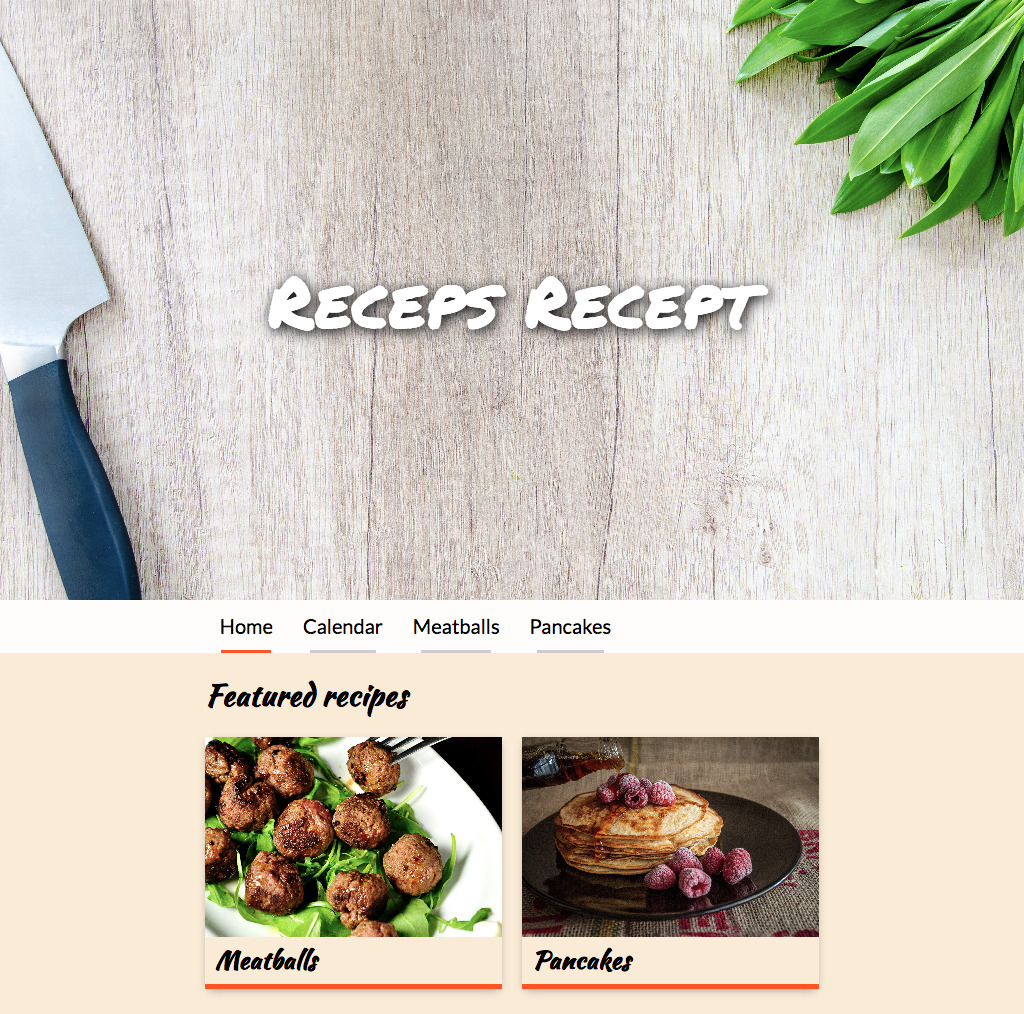
\includegraphics[width=\linewidth]{images/screenshot-index.jpg}
		\caption{Index page (Desktop)}
		\label{fig:index-page}
	\end{subfigure}
	\begin{subfigure}[b]{0.2\linewidth}
		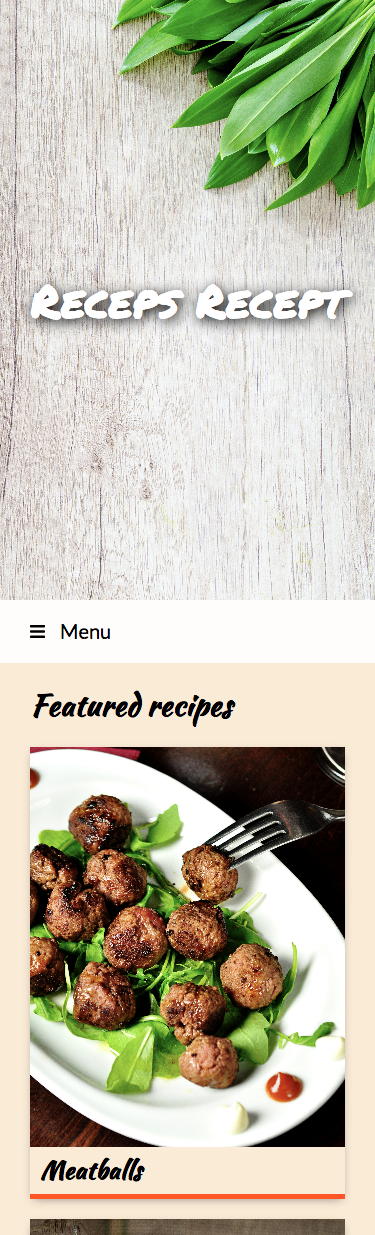
\includegraphics[width=\linewidth]{images/screenshot-index-mobile.png}
		\caption{Index page (Mobile)}
		\label{fig:index-page-mobile}
	\end{subfigure}
	\caption{Index page on different screen sizes}
\end{figure}

\begin{figure}
	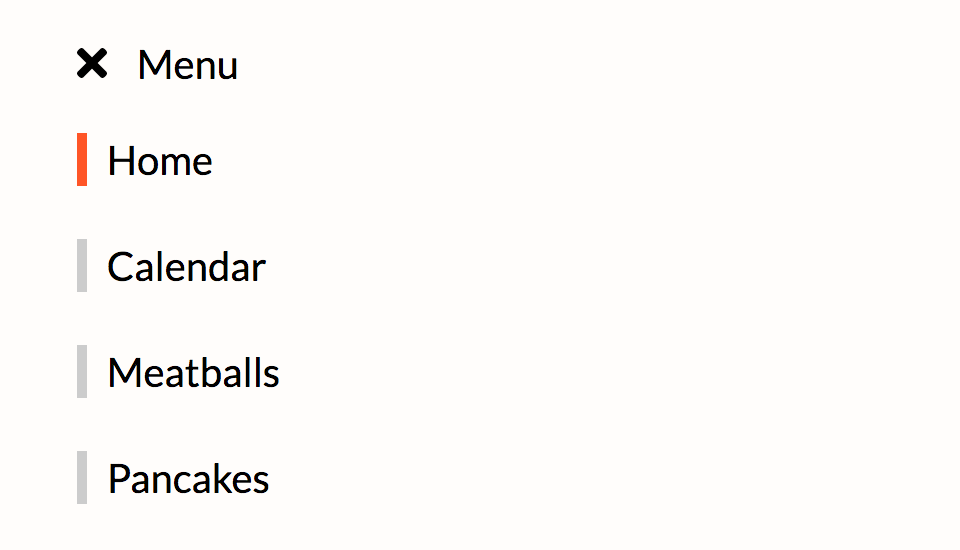
\includegraphics[width=\linewidth]{images/mobile-menu-expanded.png}
	\caption{Mobile navigation bar in expanded state}
	\label{fig:mobile-nav}
\end{figure}

\subsection{Calendar Page (design)}

As mentioned the calendar in the calendar page was inspired from another one. It was inspired on the design of a calendar created with Semantic UI. A comparison of the two is shown in figure \ref{fig:calendar-comparison}. No code was copied from the original inspiration.

\begin{figure}
	\centering
	\begin{subfigure}[b]{0.45\linewidth}
		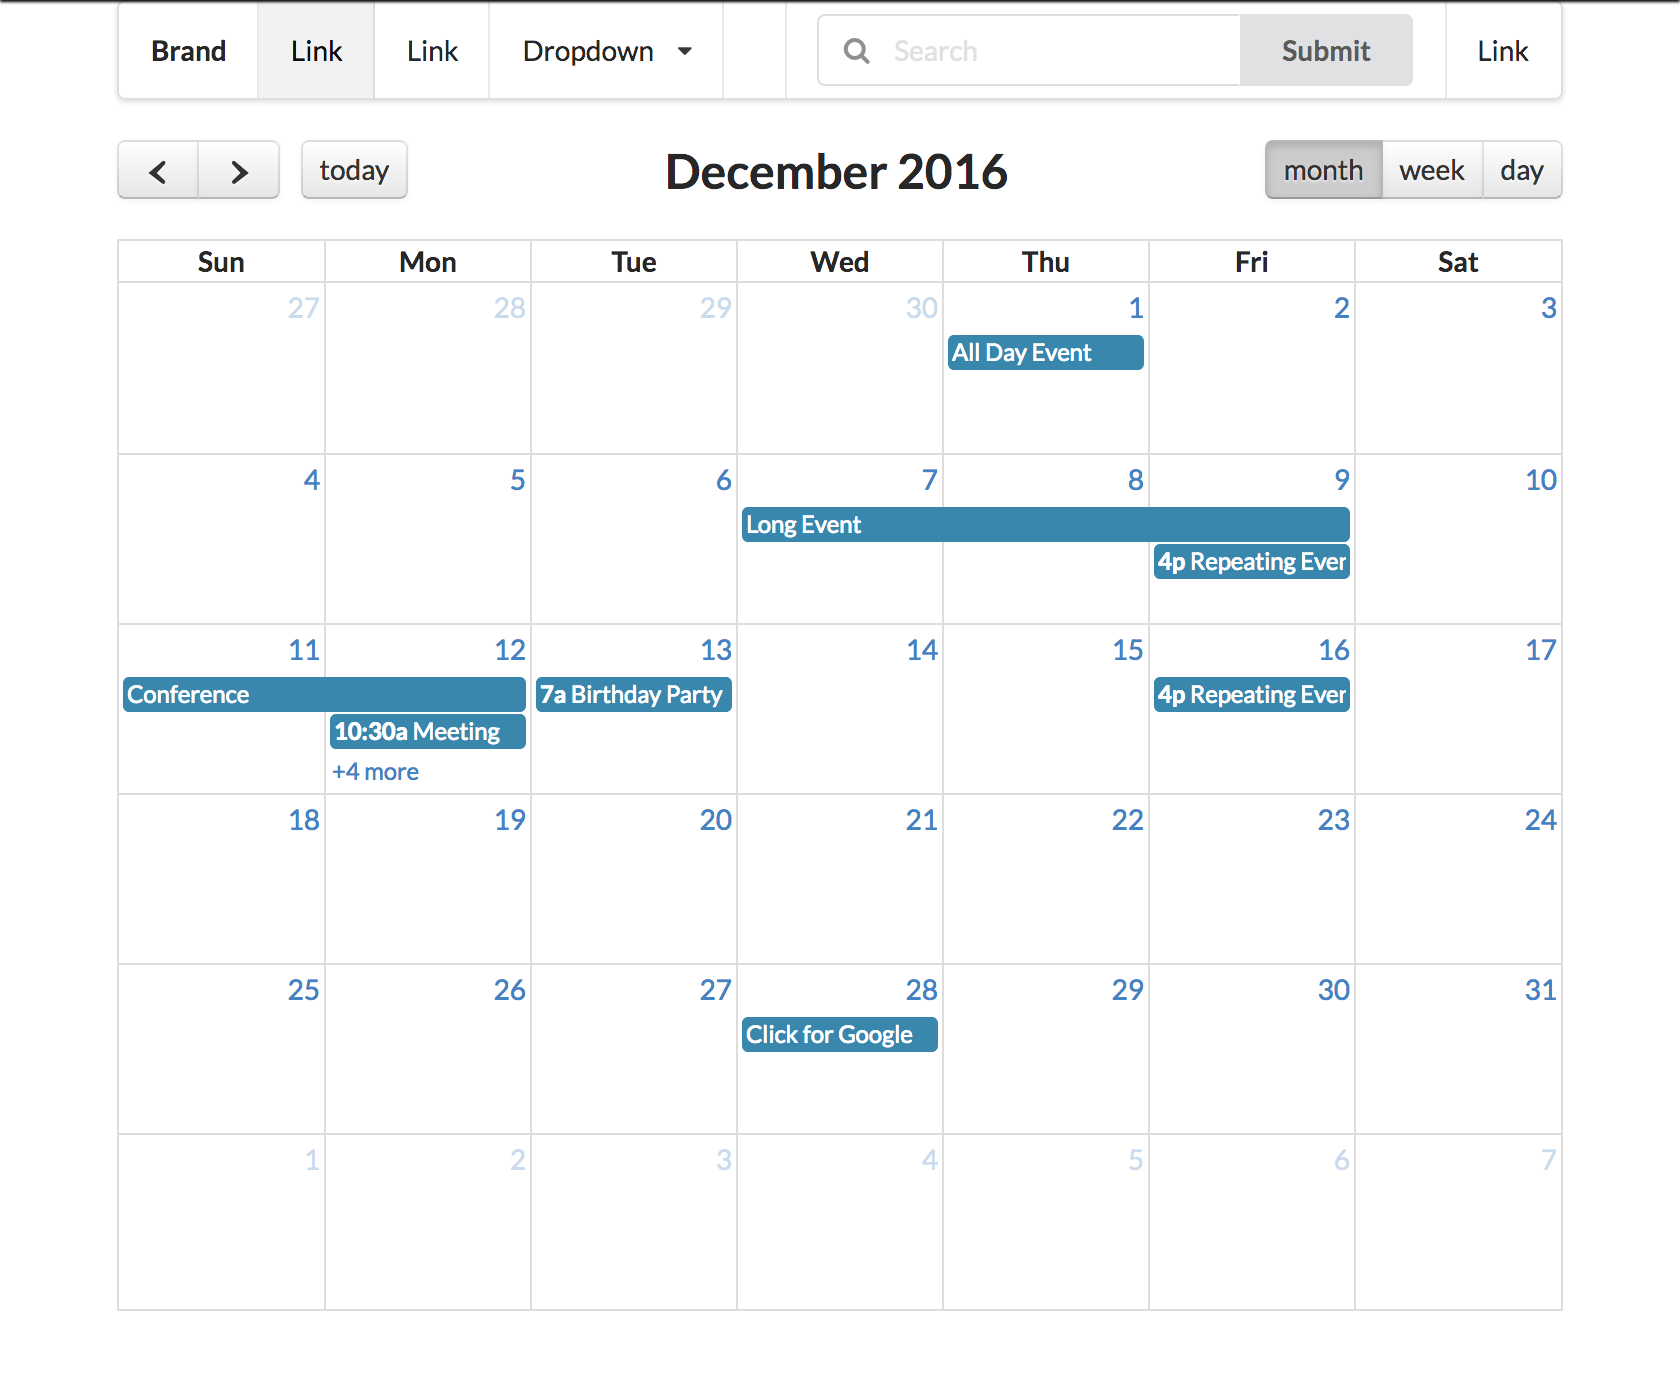
\includegraphics[width=\linewidth]{images/Semantic_UI-calendar.png}
		\caption{Semantic UI - Calendar}
	\end{subfigure}
	\begin{subfigure}[b]{0.45\linewidth}
		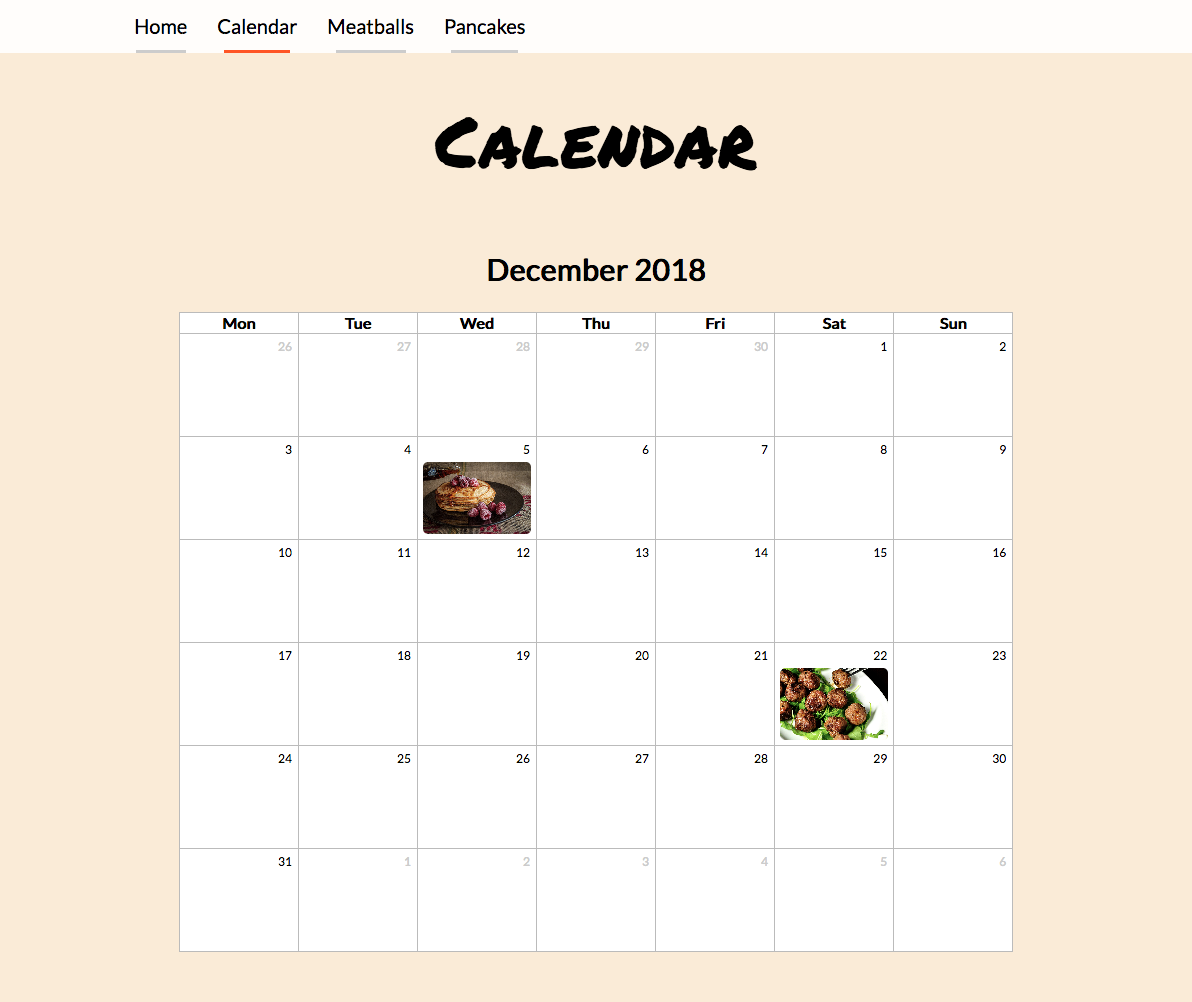
\includegraphics[width=\linewidth]{images/calendar.png}
		\caption{Receps Recept - Calendar}
	\end{subfigure}
	\caption{Calendar comparison}
	\label{fig:calendar-comparison}
\end{figure}

\subsection{Heuristics of user design}

Five of the ten basic heuristics for user interface design were considered.

\subsubsection{Visibility of system status}
The web page is mostly stateless. One of two states is the state of the navigation bar when viewing the web page with a mobile device, or a device with a very small screen. The interaction is instant so the state is always visible. The state of the navigation bar can be collapsed or expanded, which is indicated with an icon. Another state is the state of which page is open. It is indicated with a small red indicator in the navigation bar that underlines the active page.

\subsubsection{Match between system and the real world}
All of the user visible text is adapted to the users. All of the text has been proofread.

\subsubsection{Consistency and standards}
The design is simple and mostly consistent. Three fonts are used and they are always used on the same place. There is one font used only for the main header on every page. There is another font that is used for secondary headers that are not directly placed inside another element.

The position of the navigation bar is on the most top of the web page on every page except for one. On the index page it is not on the top of the page, however that is justified with the index page having a unique and inviting design. The design of the navigation bar is exactly the same on every page though.

The design of the navigation bar keeps a consistent design profile. Even though the design and layout is different on different screen sizes, there are similar visual elements that are presented. The red line that indicates what page is active is presented both on mobile and desktop screen sizes.

\subsubsection{Recognition rather than recall}
All of the user interactions are clear. Users do not have to remember information to revisit a page they previously visited, as all pages are always easy to find. Ingredients, recipe instructions and comments are all collected on the same place.

Images help users understand context. Images help users understand the recipe links on the first page. Images are also used in the calendar to clearly show which recipes are relevant for each day.

\subsubsection{Aesthetic and minimalist design}
The navigation menu adapts after screen size. When the screen is smaller less information can be presented on the screen. Therefore every piece of information is more valuable. That is why the navigation bar is fully visible on larger screens while being collapsible on smaller screens.

There are no irrelevant units of information. The design is simple. Font sizes are used to build information hierarchies to highlight important information for quick information access.

\subsubsection{Browser Consistency}
The web page was tested on multiple browsers and differences were not distinguishable without placing the browsers next to each other. The page looked quite consistent even on the Kindle Paperwhite Experimental browser. Even if the browser had no support for CSS Flexbox or CSS Grid, the parts that used those technologies failed gracefully, and the browsing experience was not severally altered. The page looked surprisingly very good on Opera Mini, which is a browser that lacks very much HTML and CSS functionality.

I did have problems with text-shadow rendering consistently, however I do not think it is possible to get that to look exactly the same, and I do not believe it is important. Figure \ref{fig:browser-comparison} shows a comparison of the pancake page on the browsers Firefox and Chrome. When I test my designs on multiple browsers, the important part is not that the web page looks exactly the same on all browsers, but it is that the web page looks good on all browsers. Sometimes I use newer features, even though I avoid them if they impact to many users, however I always ensure that the web page is usable looks good even for users who can not view the web page with all necessary features enabled.

\begin{figure}
	\centering
	\begin{subfigure}[b]{0.45\linewidth}
		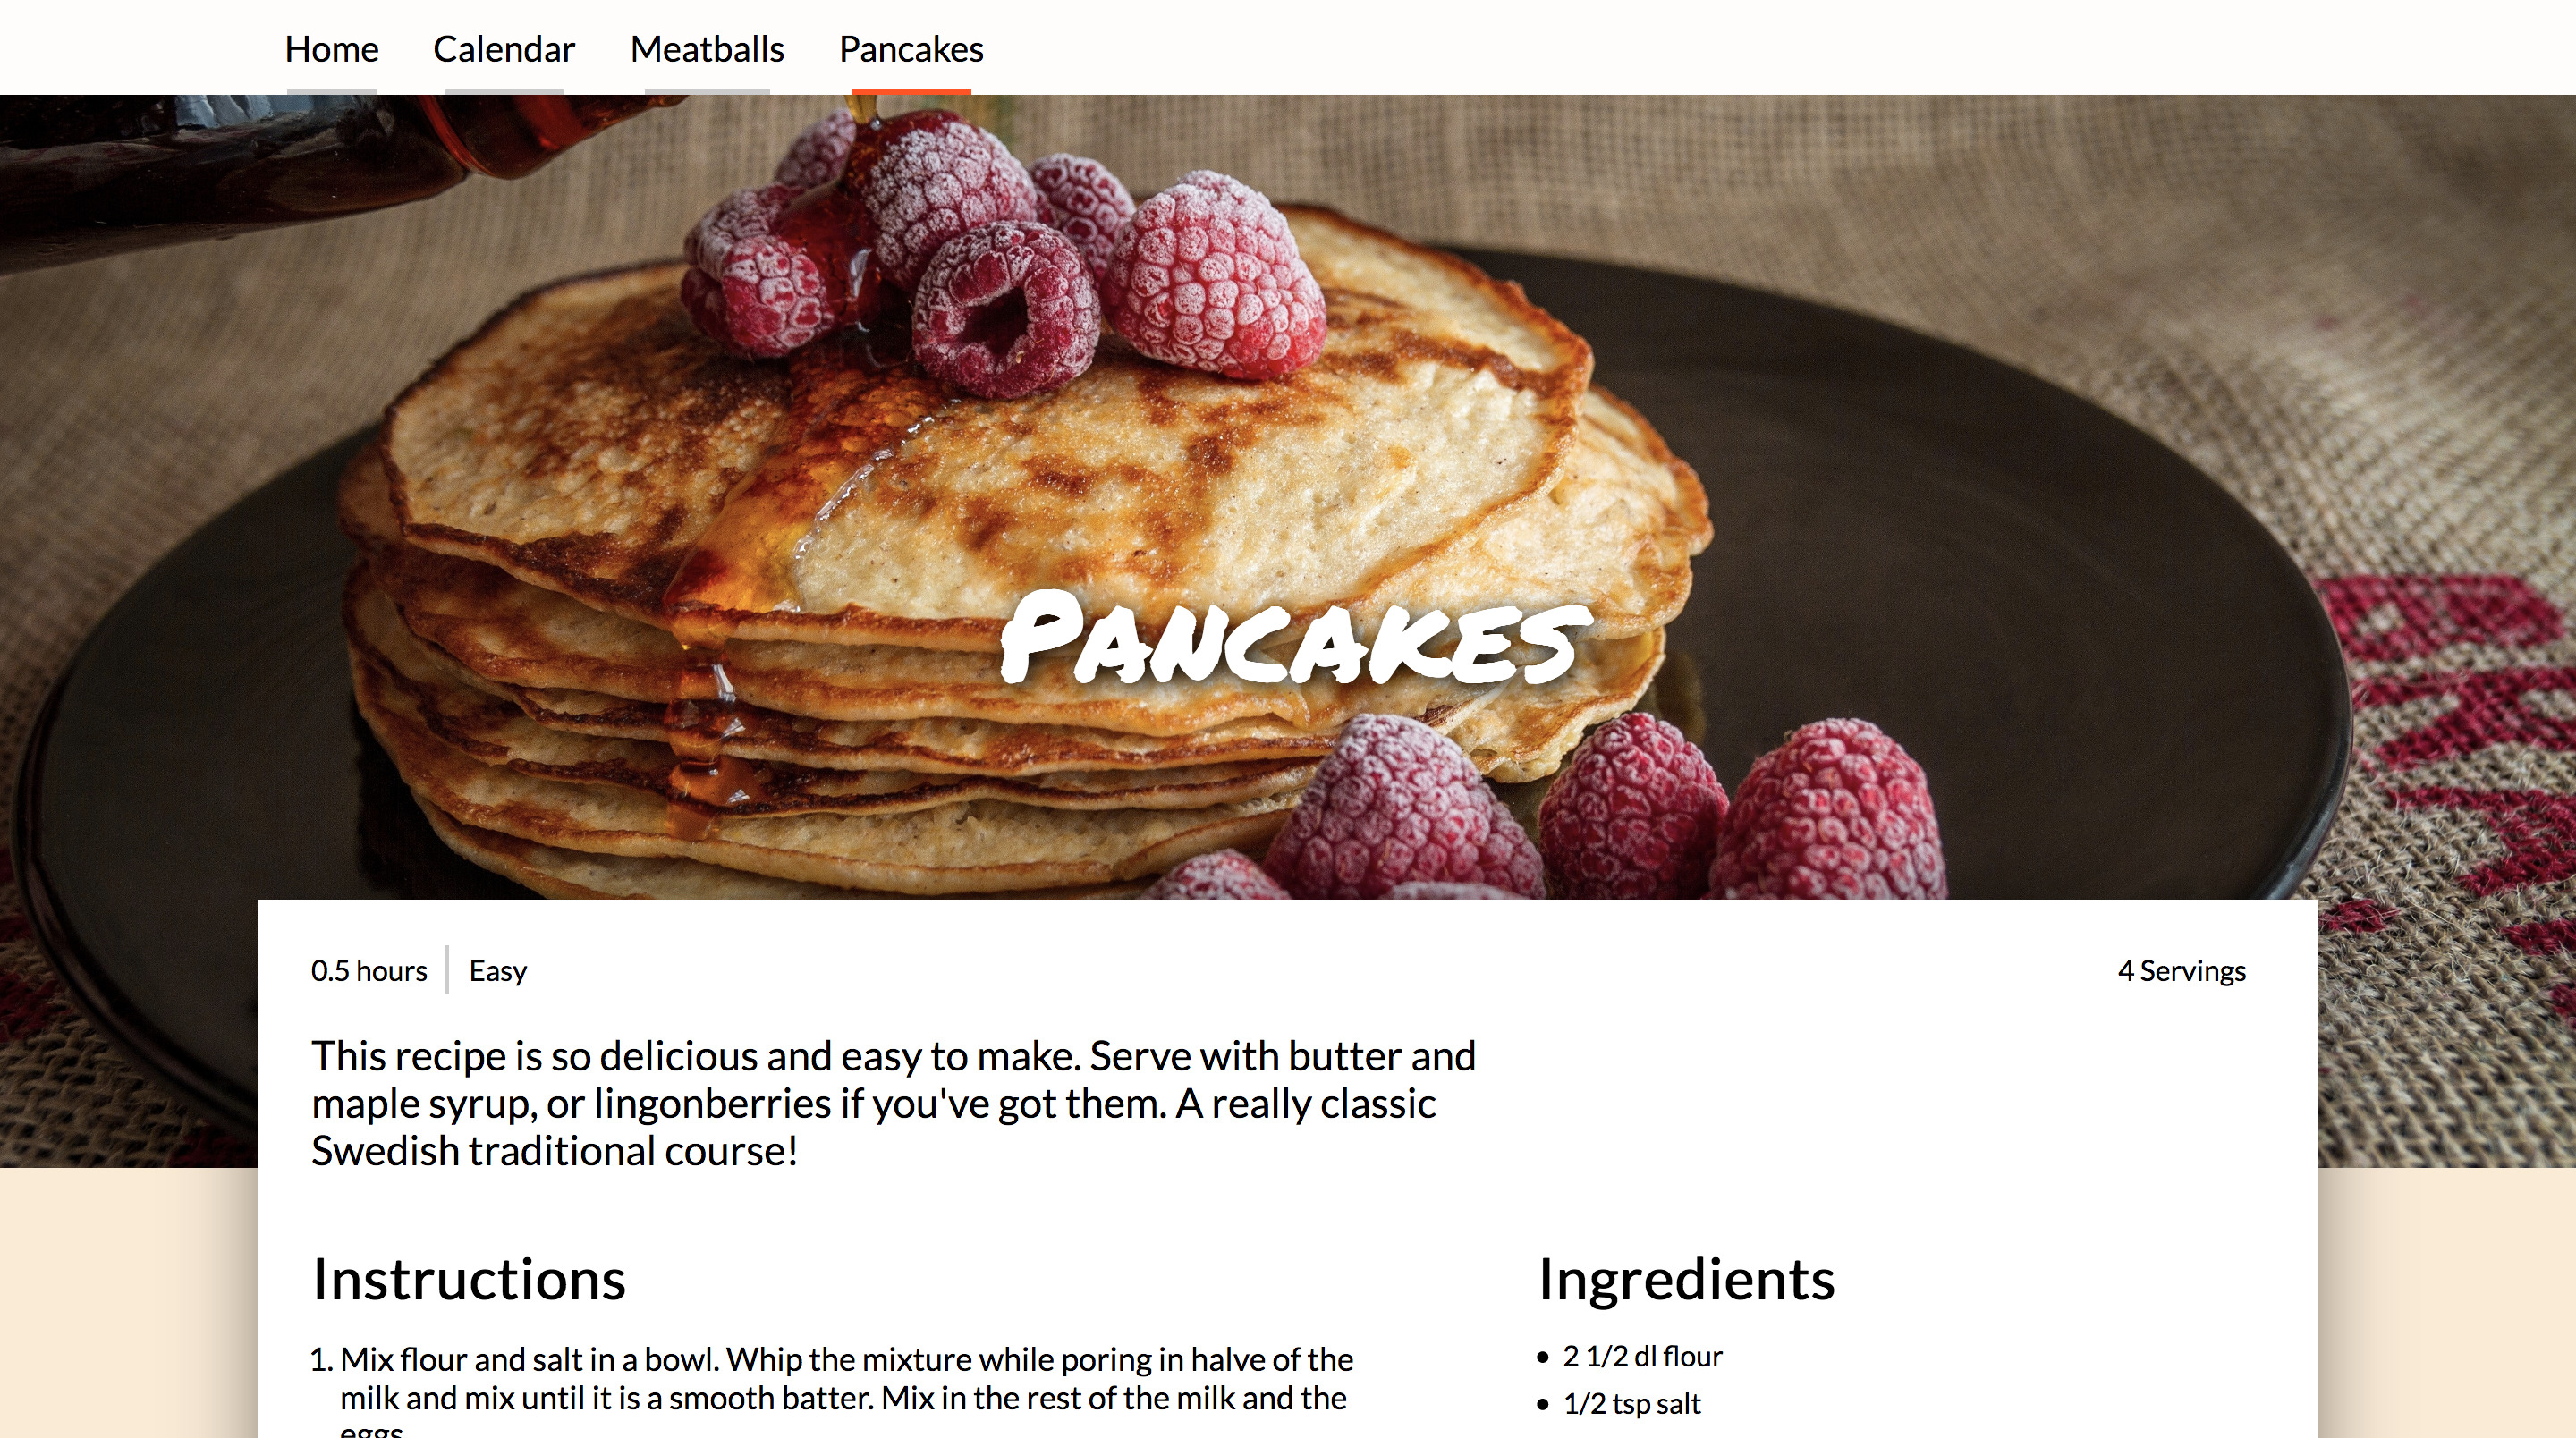
\includegraphics[width=\linewidth]{images/screen-shot-firefox.jpg}
		\caption{Pancake page in Firefox}
	\end{subfigure}
	\begin{subfigure}[b]{0.45\linewidth}
		\includegraphics[width=\linewidth]{images/screen-shot-chrome.png}
		\caption{Receps Recept - Calendar}
	\end{subfigure}
	\caption{Pancake page in Chrome}
	\label{fig:browser-comparison}
\end{figure}

\subsection{Accessibility}

There was an alt attribute for every image, ensuring that there was always a text alternative. The web page did not rely on color in any meaningful way, except for minor indicators on the navigation bar. The web page was viewed on a Amazon Kindle Paperwhite, that has a very poor screen that can not show colors. The web page was considered fully usable.

All HTML and CSS was used properly. I did not use tables for layout, and I used tables for presenting tabular data. I did use the correct \texttt{<h1> - <h6>} tags to create a structural hierarchy. I did use the \texttt{<header>} and the \texttt{<nav>} tag to indicate header and navigation bar. The page is fully usable without any CSS, and the ordering of items is correct.

There was clear navigation mechanisms where a user could clearly navigate from any page to any other page. Every link contained meaningful markup, so that they could be understood without further context.

\section{Discussion}

The mandatory requirements where:
\begin{enumerate}
	\item Create a website using HTML and CSS, ensure that all files pass the W3C Validation, use a reset CSS, and explain important parts of the code.
	\item Consider five of the ten basic heuristics for user interface design.
	\item Ensure browser consistency.
\end{enumerate}

The optional requirements where:
\begin{enumerate}
	\item The web page is responsive, adapting to multiple screen sizes and aspect ratios.
	\item The web site shall follow the four accessibility guidelines given.
\end{enumerate}


\noindent
I have met every requirement. I did get an opportunity to properly try BEM, which I have only done a little bit before. This is probably my greatest lesson from this assignment. I really like BEM and will definitively use it again. My biggest problem with the website is that the file sizes on the images are very large. It does impact load time which I would fix if this website would go into production.

\section{Comments About the Course}

I really like that feedback is collected often during the course. It makes me as a student feel appreciated, and it makes me more invested in the course. I like the assignemnts and the lectures. The course website is very clear and structured, as the rest of the course also is. It really helps us when everything is clear from the beginning. The only thing I could complain about now is that all assignments are not available yet. As the slides are available one could study in advance and it could be possible to want to start with the assignments early.

It took me about a day to create the website, and about one day to write the report.

\printbibliography[heading=bibintoc]

\end{document}
